\documentclass{beamer}
\mode<presentation> {
\usetheme{Madrid}
}
\usepackage{graphicx}
\usepackage{animate}
\usepackage{graphicx}
\usepackage{booktabs} 
\usepackage{bibentry}
\usepackage{xcolor}
\usepackage{enumitem}

\title[ADMM]{Alternating direction method of multipliers (ADMM) algorithm for solving bi-clustering problem: application to microbiome data analysis} 
\author{Lanqiu Yao} 
\institute[NYU] 
{
NYU School of Medicine \\
Division of Biostatistics\\ 
\medskip
\textit{ly1192@nyu.edu} 
}
\date{May 8, 2019} 




\begin{document}

%1
\begin{frame}
\titlepage 
\end{frame}

%2
\begin{frame}
\frametitle{Overview} 
\tableofcontents 
\end{frame}

\section{Introduction}
\subsection{Bi-clustering problem}

%3
\begin{frame}
\frametitle{Introduction: Clustering}

Clustering is the task of grouping a set of objects in such a way that objects in the same group (called a cluster) are more similar (in some sense) to each other than to those in other groups (clusters)
\vfill
Pattern recognition
\begin{itemize}
    \item Cells: Prokaryotic cells, Eukaryotic cells...
    \item Lung cancer: Lung adenocarcinoma, Squamous cell carcinoma, Small cell carcinoma,. Large cell carcinoma ...
    \item Restaurant: good restaurant, bad restaurant. 
\end{itemize}

Method: 
\begin{itemize}
    \item Hierarchical clustering
    \item K-means
    \item ...
\end{itemize}

\end{frame}

\begin{frame}{Introduction: Biclustering}
    The previously mentioned clustering methods can only identify one kinds of features. 
    
    Some times people want to cluster the observations and features simultaneously. Then biclustering algorithms are needed. 
    
    \begin{itemize}
        \item smoking/nonsomking
        \item lung cancer/health
    \end{itemize}
    
    Biclustering has applications in a wide world. It can help people identify subsets of genes/ microbiome within subsets of conditions.
    
    \centering
    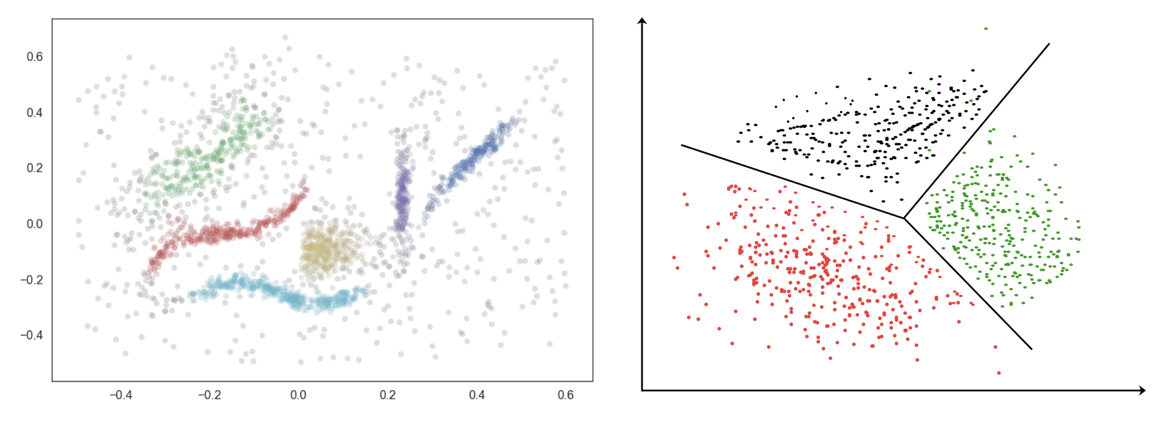
\includegraphics[width=10cm,height=5cm,keepaspectratio]{cluster}
    
\end{frame}

%4
\subsection{Microbiome clustering}
\begin{frame}
\frametitle{Introduction: Microbiome clustering}

The Effect of Diet on the Human Gut Microbiome \footnote{Turnbaugh, Peter J., et al. "The effect of diet on the human gut microbiome: a metagenomic analysis in humanized gnotobiotic mice." Science translational medicine 1.6 (2009): 6ra14-6ra14.}

\vfill

  \centering
    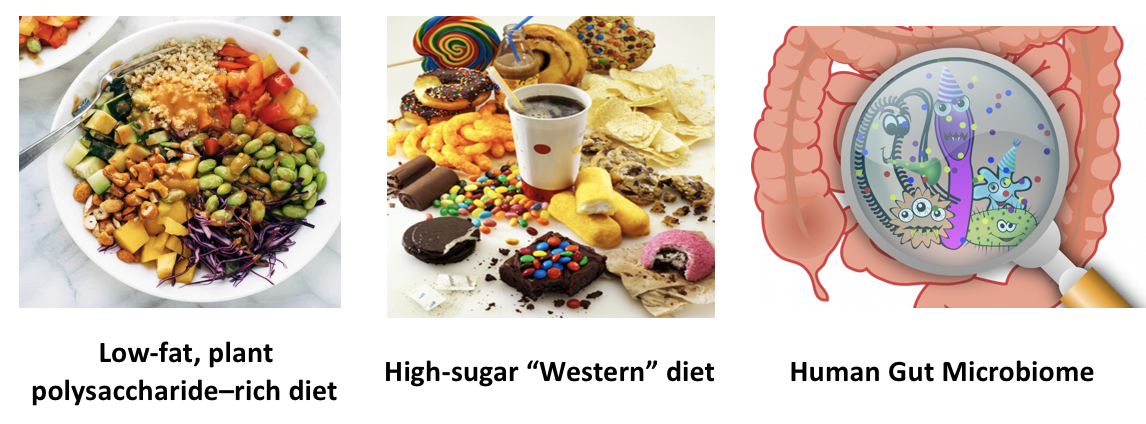
\includegraphics[width=12cm,height=6cm,keepaspectratio]{diet}
    
\end{frame}


\section{Algorithm}
\subsection{ADMM}

%5
\begin{frame}{ADMM}

\begin{itemize}
    \item ADMM
\end{itemize}

    Alternating direction method of multipliers(ADMM) is an algorithm that is intended to blend the decomposability
of dual ascent with the superior convergence properties of the method
of multipliers. The algorithm solves problems in the form
$$\text{min} f(x) + g(z)$$
$$Ax + Bz = 0$$
with variable $x \in R^n$, $z \in R^m$, where $A \in R^{p \tims n}$, $B \in R^{p \times m}$, and $C \in R^p$
\vfill
Let's look at the biclustering ADMM algorithm 

\end{frame}



%6
\begin{frame}
\frametitle{ADMM}
\begin{itemize}
    \item $X$ is an $n \times p$ matrix, with $n$ observations and $p$ features.
\end{itemize}
 
$$\mathbf{X}_{n,p} = \left[\begin{array}
{rrrr}
X_{11} & X_{12} & ... & X_{1p}\\
X_{21} & X_{22} & ... & X_{2p}\\
... & ... & ... & ... \\
X_{n1} & X_{n2} & ... & X_{np}
\end{array}\right] = (X_{\cdot 1}, X_{\cdot 2},..., X_{\cdot p})$$

\begin{itemize}
    \item Assume that the $n$ observations belong to $R$ unknown and non-overlape classes. 
    \item Assume that the $p$ features belong to $C$ unknown and non-overlap classes.
    \item Cluster mean: $\mathbf{\mu} = \{\mu_{r,c}\} \in \mathbb{R}^{R \times C}$
    \item Cluster mean: $\mu_{r,c} = \frac{1}{|R||C|} \sum_{i \in R, j \in C} x_{ij}$
    \item Let $A = \{a_{ij}\} \in \mathbb{R}^{n \times p}$, where $A$ matrix is the estimated the cluster labels/pattern of matrix $X$
\end{itemize}
\end{frame}



% 7
\begin{frame}
\frametitle{ADMM}
The convex biclustering problem can be formulated as:
$$\text{min}_{A \in \mathbb{R}^{n \times p}}  \frac{1}{2} \sum^p_{i=1} ||X_{\cdot i} - A_{\cdot i}||_2^2 + \gamma_1 \sum_{ l \in E_1 } w_{l} ||\mathbf{v}_l||_{q} + \gamma_2 \sum_{k \in E_2 } u_{k} ||\mathbf{z}_k||_{q}$$
$$s.t. \text{ } A_{l_1 \cdot} - A_{l_2 \cdot} - \mathbf{v}_l = 0$$
\begin{equation}
    A_{\cdot k_1 } - A_{\cdot k_2} - \mathbf{z}_k = 0 \tag{*}
\end{equation}

where,
\begin{itemize}
    \item $E_1 = \{l = (l_1, l_2): 1 \leq l_1 < l_2 \leq n\}$
    \item $E_2 = \{k = (k_1, k_2): 1 \leq k_1 < k_2 \leq n\}$
    \item $|| \cdot ||_q$ is the $L_q$ norm, $q$ can be $1, 2,..., \text{or } \infty$
\end{itemize}
\end{frame}


% 8
\begin{frame}
\frametitle{ADMM}
Let's see an example: 
\vfill
$\mu_{1,1} = 1.5, \mu_{1,2} = -2, \mu_{2,1} = -1.5
, \mu_{2,2} = 2$
\centering
\animategraphics[width=0.6\linewidth,autoplay,controls]{8}{a}{1}{4}
\end{frame}

%9
\begin{frame}
\frametitle{ADMM}
Let's see an example: 

$\mu_{1,1} = 1.5, \mu_{1,2} = -2, \mu_{2,1} = -1.5
, \mu_{2,2} = 2$

\centering
    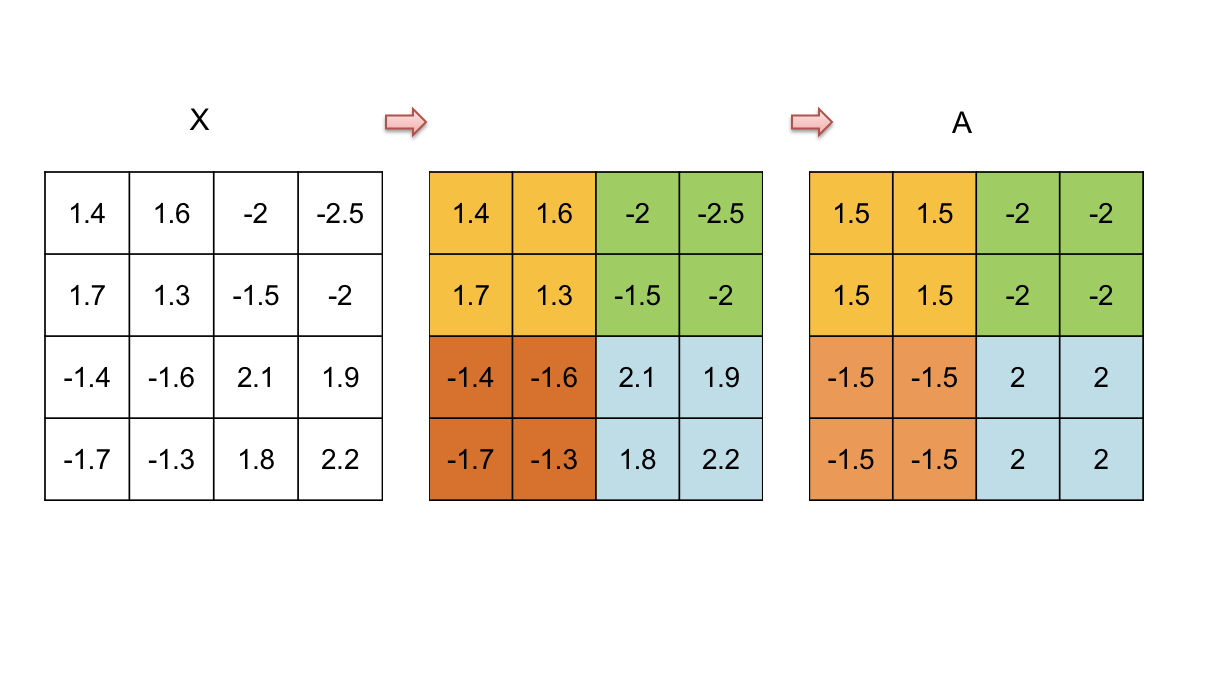
\includegraphics[width=12cm,height=6cm,keepaspectratio]{a4}
\end{frame}

%10
\subsection{Augmented Lagrangian Method}
\begin{frame}{ADMM}
To solve this constrained optimization problem we can use augmented Lagrangian method:
$$
\begin{aligned}
\mathcal{L}_{\nu_1,\nu_2}(A,V,Z,\Lambda_1, \Lambda_2) = & \frac{1}{2} \sum^p_{i=1} ||X_{\cdot i} - A_{\cdot i}||_2^2 + \gamma_1 \sum_{ l \in E_1 } w_{l} ||\mathbf{v}_l||_{q} \\
 & + \gamma_2 \sum_{k \in E_2 } u_{k} ||\mathbf{z}_k||_{q} + \\
  & \sum_{l \in E_1}<\lambda_{1l},\mathbf{v}_l - A_{l_1 \cdot} + A_{l_2 \cdot} > \\
  & +  \frac{\nu_1}{2} \sum_{l \in E_1} ||\mathbf{v}_l - A_{l_1 \cdot} + A_{l_2 \cdot}||_2^2 \\
  & + \sum_{k \in E_2}<\lambda_{2k},\mathbf{z}_k - A_{\cdot k_1 } + A_{\cdot k_2} > \\
  &+ \frac{\nu_2}{2}\sum_{k \in E_2} || \mathbf{z}_k - A_{\cdot k_1 } + A_{\cdot k_2}||_2^2
\end{aligned}
$$
\end{frame}


% 11
\begin{frame}{ADMM}

Parameters:
\begin{itemize}
    \item  $\nu_1, \nu_1 , \gamma_1, \gamma_2$
    \item Need to solve: $A$
\end{itemize}
Iterations: 
\begin{itemize}
    \item Update $A$
    \item Update $\mathbf{V}, \mathbf{Z}$
    \item Update $\Lambda_1$, $\Lambda_2$
\end{itemize}
\end{frame}

% 12
\begin{frame}{ADMM - Update A}
    It is the most challenging part. We need to minimize 

$$
\begin{aligned}
    f(A) =& \frac{1}{2} \sum^p_{i=1} ||X_{\cdot i} - A_{\cdot i}||_2^2  \\
     & + \frac{\nu_1}{2}\sum_{l \in E_1} ||\tilde{\mathbf{v}_l} - A_{l_1 \cdot} + A_{l_2 \cdot} ||^2_2 \\
     & + \frac{\nu_2}{2} \sum_{k \in E_2} ||\tilde{\mathbf{z_k}} - A_{\cdot k_1 } + A_{\cdot k_2}||^2_2   
\end{aligned}
$$    
    where,
    \begin{itemize}
        \item $\tilde{\mathbf{v_l}} = \mathbf{v_l} + \frac{1}{\nu_1} \lambda_{1l}$
        \item $\tilde{\mathbf{z_k}} = \mathbf{z_k} + \frac{1}{\nu_2} \lambda_{2k}$
    \end{itemize}
\end{frame}

% 13
\begin{frame}{ADMM - Update A}

We could calculate its derivation. And the system of equations is finally equivalent to a Sylvester equation:
\begin{equation}
    MA + AN = C \tag{1}
\end{equation}
where, 
\begin{equation}
    M = I_n + \nu_1 \sum_{l \in E_1}(e_{l_1} - e_{l_2})(e_{l_1} - e_{l_2})^T \tag{2}
\end{equation}

\begin{equation}
    N = \nu_2 \sum_{k \in E_2}(e^{*}_{k_1} - e^{*}_{k_2})(e^{*}_{k_1} - e^{*}_{k_2})^T \tag{3}
\end{equation}

\begin{equation}
    C = X + \sum_{l in \E_1} (e_{l_1} - e_{l_2})(\lambda_{1l} + \nu_1 \mathbf{v_l})^T    + (\lambda_{2k} + \nu_2 \mathbf{z_k}) (e^{*}_{k_1} - e^{*}_{k_2})^T \tag{4}
\end{equation}

where $A_{l_1 \cdot} + A_{l_2 \cdot} = A(e_{l_1} - e_{l_2})$, $e_{l_1}$ and $e_{l_2}$ are $p \times 1$ vectors. 

And similarly, $A_{\cdot k_1 } + A_{\cdot k_2} = A^T(e^{*}_{k_1} - e^{*}_{k_2})$, $e^{*}_{k_1}$ and $e^{*}_{k_2}$ are $n \times 1$ vectors.

\end{frame}

% 14
\begin{frame}{Sylvester equation}
  
    Algorithm for solving Sylvester equation: 
     Bartels–Stewart algorithm
     \footnote{Sorensen, Danny C., and Yunkai Zhou. "Direct methods for matrix Sylvester and Lyapunov equations." Journal of Applied Mathematics 6.2003 (2003): 277-303.}
    
    \centering
    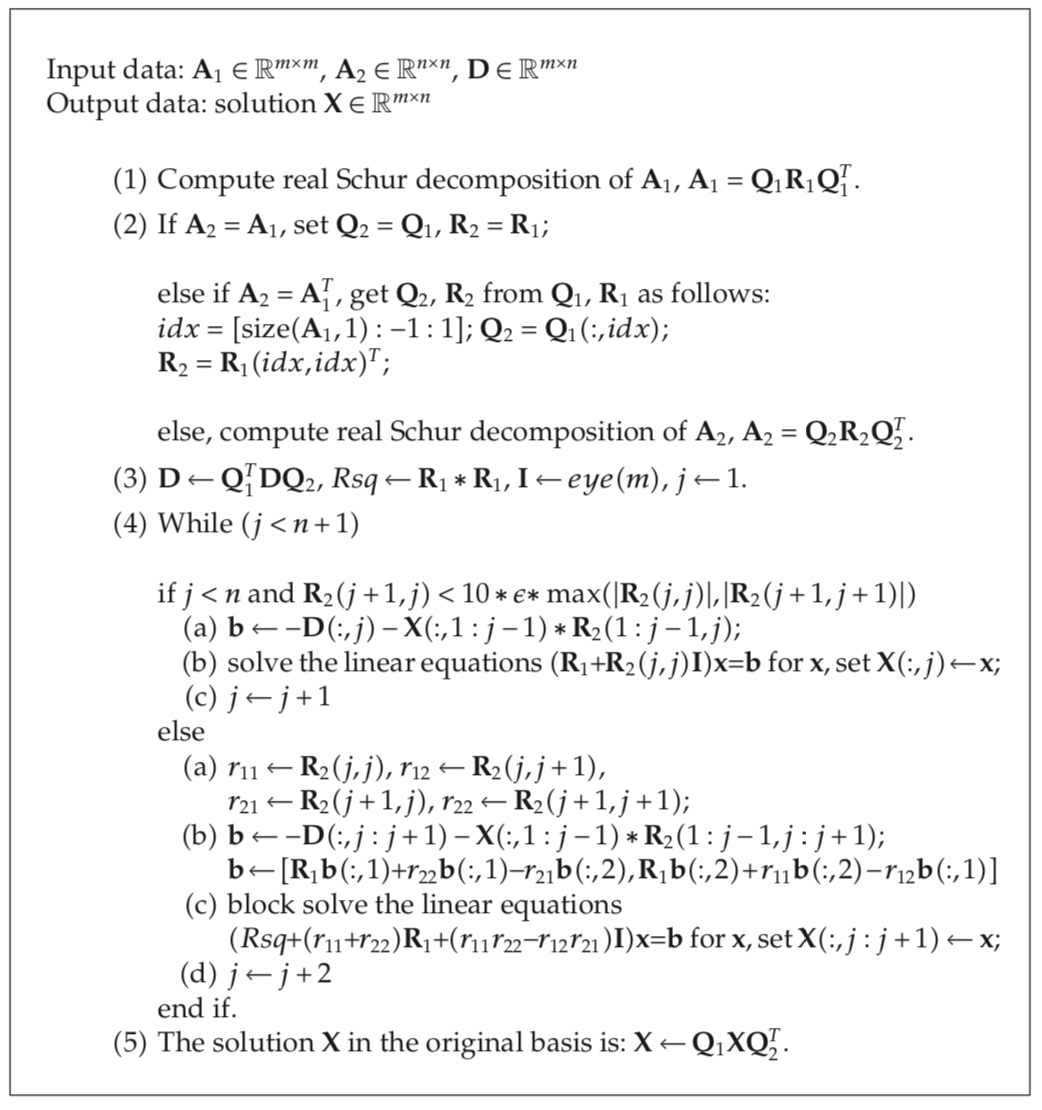
\includegraphics[width=12cm,height=6cm,keepaspectratio]{eq}
    
\end{frame}

% 15
\begin{frame}{ADMM - Update V,Z}
Proximal maps \footnote{Chi, Eric C., and Kenneth Lange. "Splitting methods for convex clustering." Journal of Computational and Graphical Statistics 24.4 (2015): 994-1013.}
    $$
    \begin{aligned}
       \mathbf{v}_l &= \text{argmin}_{\mathbf{v}_l} \frac{1}{2} ||\mathbf{v}_l - (A_{l_1 \cdot} - A_{l_2 \cdot} + \nu_1^{-1}\lambda_{1l})||_2^2 + \frac{\gamma_1 w_l}{\nu_1} ||\mathbf{v}_l ||_q \\
       & = prox_{\delta_{1l} ||\cdot||_q} (A_{l_1 \cdot} - A_{l_2 \cdot} + \nu_1^{-1}\lambda_{1l}) \label{5}
    \end{aligned}
 $$

$$
\begin{aligned}
       \mathbf{z}_k &= \text{argmin}_{\mathbf{z}_k} \frac{1}{2} ||\mathbf{z}_k - (A_{\cdot k_1 } - A_{\cdot k_2} + \nu_2^{-1}\lambda_{2k})||_2^2 + \frac{\gamma_2 u_k}{\nu_2} ||\mathbf{z}_k ||_q \\
       & = prox_{\delta_{2k} ||\cdot||_q} (A_{\cdot k_1 } - A_{\cdot k_2} + \nu_2^{-1}\lambda_{2k}) \lable{6}
    \end{aligned}
$$    
    
\centering
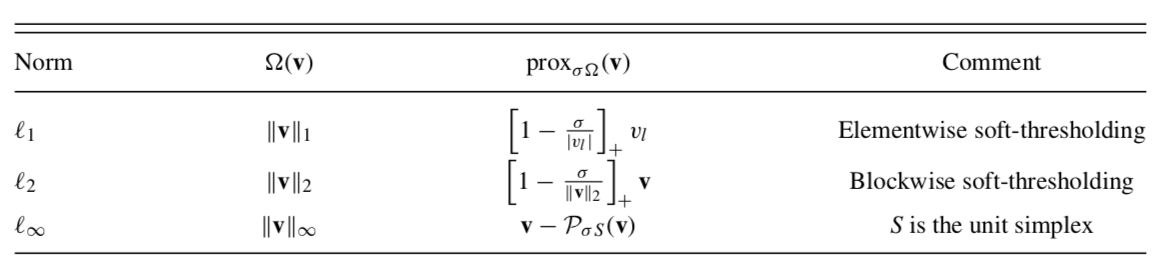
\includegraphics[width=12cm,height=6cm,keepaspectratio]{prox}
    
\end{frame}


% 16
\begin{frame}{ADMM - Update $\Lambda$}
    
    It is easy to update $\lambda_{1l}$ and $\lambda_{2k}$ 
    
    \begin{equation}
        \lambda_{1l} = \lambda_{1l} + \nu_1 (\mathbf{v}_l - A_{l_1 \cdot} + A_{l_2 \cdot}) \tag{7}
    \end{equation}
    
    \begin{equation}
        \lambda_{2k} = \lambda_{2k} + \nu_2 (\mathbf{z}_k - A_{\cdot k_1 } + A_{\cdot k_2}) \tag{8}
    \end{equation}
    
\end{frame}


\begin{frame}{ADMM}
    \centering
    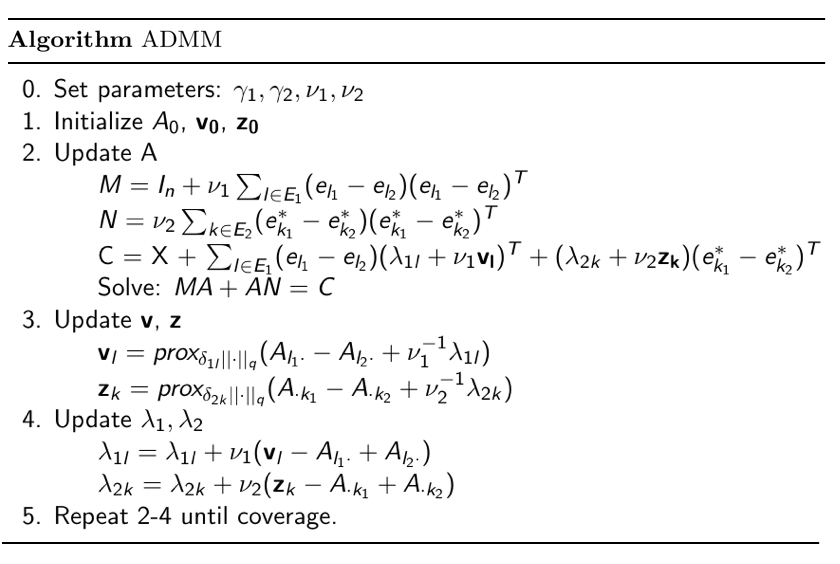
\includegraphics[width=12cm,height=6cm,keepaspectratio]{algo}
\end{frame}



\subsection{Comparison-COBRA}

\begin{frame}{Comparison}
    Compare ADMM to other bi-clustering method.
    
    Here, I would like to compare it with Convex BiclusteRing Algorithm (COBRA)\footnote{Chi, Eric C., and Kenneth Lange. "Splitting methods for convex clustering." Journal of Computational and Graphical Statistics 24.4 (2015): 994-1013.}
    
    
\end{frame}

\begin{frame}{COBRA}
    \begin{itemize}
        \item Convex BiclusteRing Algorithm (COBRA)
    \end{itemize}
     
    The method also focused on solving the Lagrangian equation. 
    
    But instead of solving the Sylvester equation, an approximate method is applied. 
    
    \begin{equation}
    MA + AN = C \tag{1}
\end{equation}
  That is, when updating $A$, $\nu_1$ and $\nu_2$ are temporally set as 0.   
  Then
  $$M = I_n, N = 0$$
  $$A = C = X + \sum_{l in \E_1} (e_{l_1} - e_{l_2})(\lambda_{1l} + \nu_1 \mathbf{v_l})^T    + (\lambda_{2k} + \nu_2 \mathbf{z_k}) (e^{*}_{k_1} - e^{*}_{k_2})^T $$

\end{frame}


\subsection{Complexity}

\begin{frame}{Complexity}
 The complexity of ADMM.
 
 \vfill
 
 For each iteration:
 
 1. Update $A$
 \begin{itemize}
     \item Calculate $M,N,C$:  $\mathcal{O}(n)$
     \item Solve Sylvester equation by Bartels–Stewart algorithm\footnote{Sorensen, Danny C., and Yunkai Zhou. "Direct methods for matrix Sylvester and Lyapunov equations." Journal of Applied Mathematics 6.2003 (2003): 277-303.}: $\mathcal{O}(n^{3})$
 \end{itemize}
 
 2. Update $\mathbf{v,z}$
 \begin{itemize}
     \item  $\mathcal{O}(n)$
 \end{itemize}
 
 3. Update $\Lambda_1, \Labmda_2$
  \begin{itemize}
     \item  $\mathcal{O}(n)$
 \end{itemize}
 
Therefore the time complexity is $\mathcal{O}(n^{3})$ for each iteration.
\vfill
The iteration numbers are usually not sure. But the algorithm will converage finally in the end. 

\end{frame}




\section{Results}

\begin{frame}{Results}
    Results:
    \begin{itemize}
        \item Simulation
        \item Microbiome data
    \end{itemize}
\end{frame}


\subsection{Simulation}


\begin{frame}{Simulation}
    Data generation: 
    
    \begin{itemize}
        \item $n \times p = 80 \times 60$
        \item $4$ clusters: $2$ row clusters and $2$ 
        \item cluster means: $\mu = [1,2,-1,-2]$
        \item cells: $x_ij \sim N(\mu, \sigma)$, $\sigma = 1$
    \end{itemize}
\end{frame}


\begin{frame}{Simulation}

Results - Heatmaps
\centering
    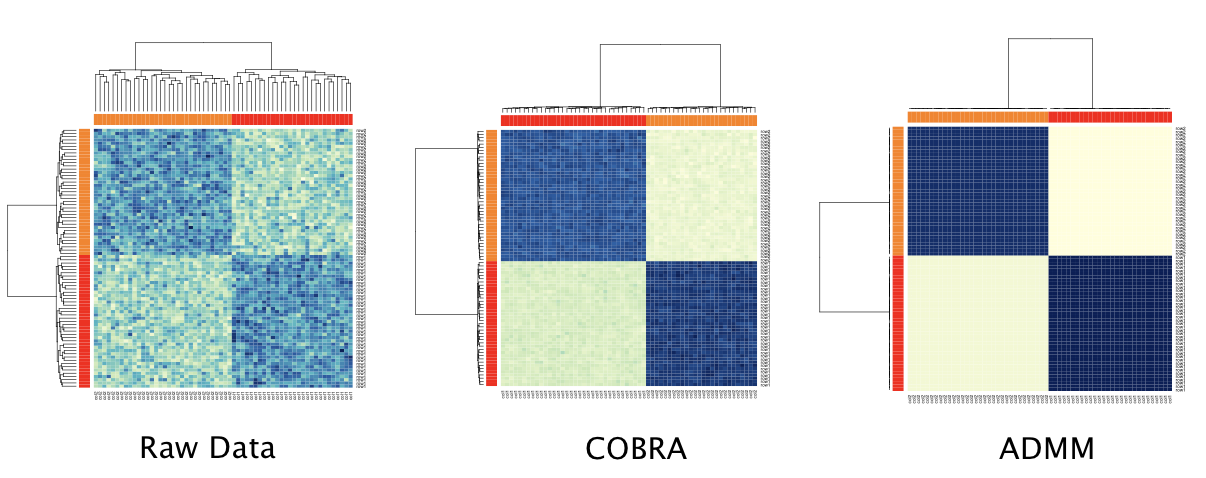
\includegraphics[width=12cm,height=6cm,keepaspectratio]{sim}
\end{frame}

\subsection{Microbiome data}

\begin{frame}{Microbiome}
The brief experiment: 
    \centering
    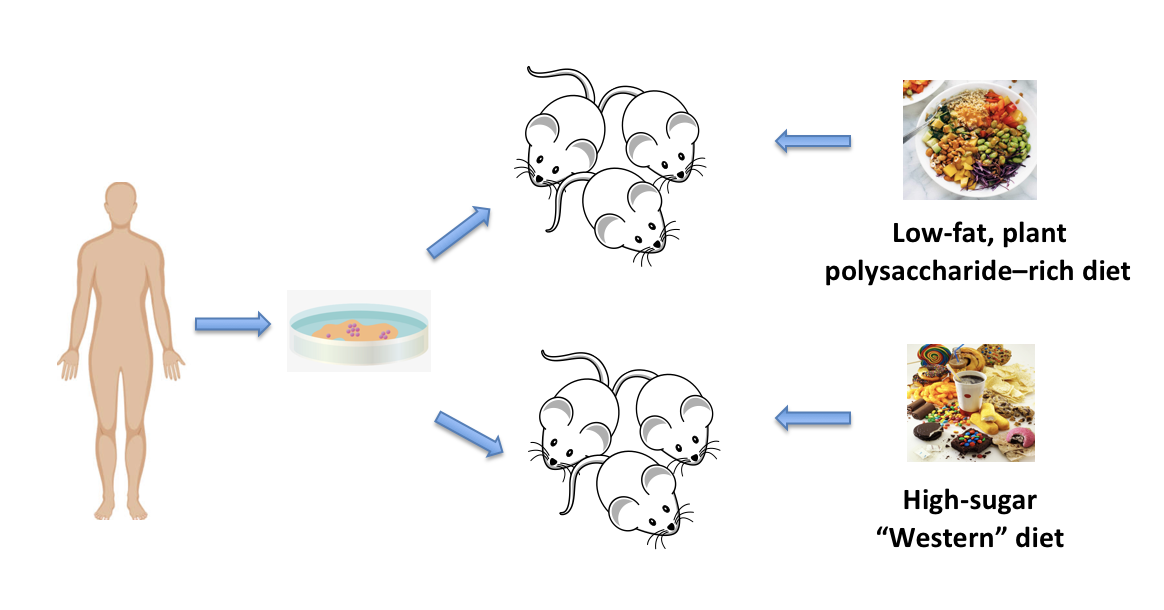
\includegraphics[width=12cm,height=6cm,keepaspectratio]{exp}
    
    The effect of diet on the microbiome?
    
\end{frame}

\begin{frame}{Microbiome}
    After 4 weeks, the sequencing of the 16S ribosomal RNA (rRNA) genes was done. 
    
    The bacterial taxa relative abundance is showing below:
    \centering
    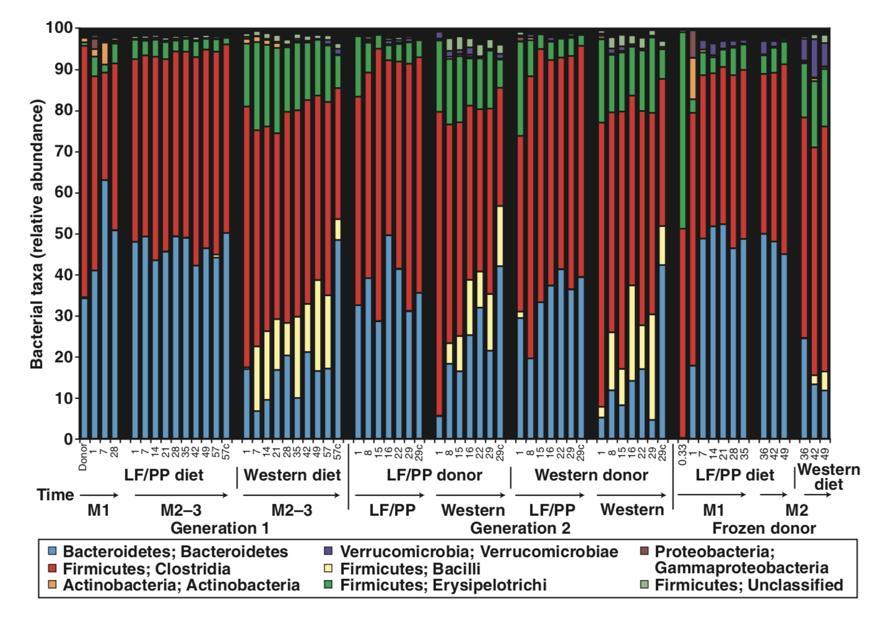
\includegraphics[width=12cm,height=6cm,keepaspectratio]{r1}
    
\end{frame}
 
\begin{frame}{Microbiome}

To make it easy, I chose the two most abundance bacterial family: 

\begin{itemize}
    \item Clostridia
    \item Bacteroidetes
\end{itemize}

In their dataset, $X = 172 \times 48$

$172$ mice and $48$ kinds of bacteria that belong to the above two families.

\vfill
\centering
    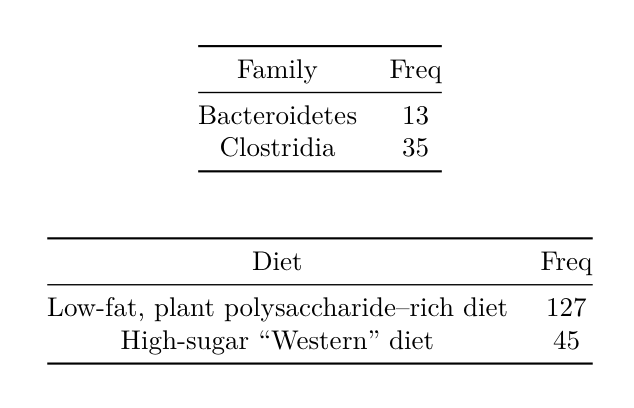
\includegraphics[width=10cm,height=5cm,keepaspectratio]{freq}
    
\end{frame}



\begin{frame}{Microbiome}
Results - Heatmaps
\centering
    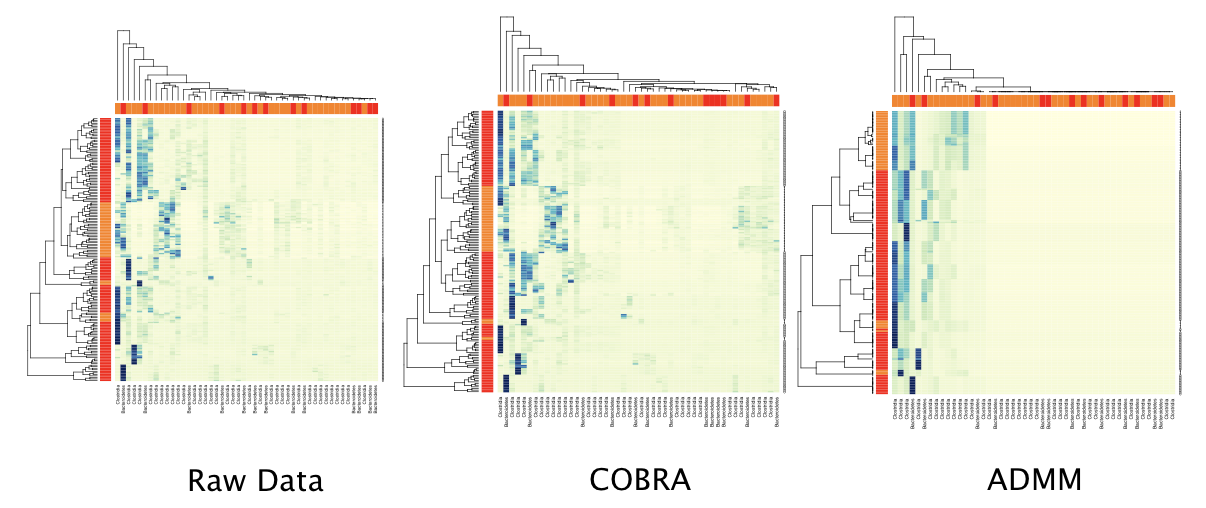
\includegraphics[width=12cm,height=6cm,keepaspectratio]{real}
\end{frame}


\section{Conclusion}

\begin{frame}{Conclusion}
    
    \begin{itemize}
        \item Biclustering algorithms can cluster the observations and features simultaneously.
        \item ADMM algorithm works better than COBRA since it get the exact solution of the augmented Lagrangian problem while COBRA gives an approximate estimator.
        \item The selection of the tuning parameters in convex clustering is important 
        \item Time complexity
    \end{itemize}
\end{frame}

\begin{frame}{Reference}
    [1] Turnbaugh, Peter J., et al. "The effect of diet on the human gut microbiome: a metagenomic analysis in humanized gnotobiotic mice." Science translational medicine 1.6 (2009): 6ra14-6ra14.
    
    [2] Chi, Eric C., Genevera I. Allen, and Richard G. Baraniuk. "Convex biclustering." Biometrics 73.1 (2017): 10-19.
    
    [3] Sorensen, Danny C., and Yunkai Zhou. "Direct methods for matrix Sylvester and Lyapunov equations." Journal of Applied Mathematics 6.2003 (2003): 277-303.
    
    [4] Chi, Eric C., and Kenneth Lange. "Splitting methods for convex clustering." Journal of Computational and Graphical Statistics 24.4 (2015): 994-1013.
    
    [5] Chi, Eric C., and Kenneth Lange. "Splitting methods for convex clustering." Journal of Computational and Graphical Statistics 24.4 (2015): 994-1013.

\end{frame}


\begin{frame}
\centering
Thank you!

\end{frame}


\end{document}